\chapter{Theoretical background}
\label{chap1} % id kapitoly pre prikaz ref

\section{Implicit surfaces}
\label{sub2.1}

Implicit functions are a tool for surface representation and manipulation.
In computer graphics, they can be used for modelling of complex surfaces
using boolean operations, realistic animations, rendering and other.

Implicit functions do not define the surface explicitly, instead
the surface is defined as a zero set of a function.
\begin{definition}
    Given a function $F: \R^3 \to \R$, one can define an implicit surface
    as a set of points $(x, y, z)\in \R^3$ that satisfy $F(x, y, z) = 0$.
\end{definition}

Some examples of implicit surfaces and their equations can be seen on
the Figure \ref{img:1}.

\begin{figure}
    \centerline{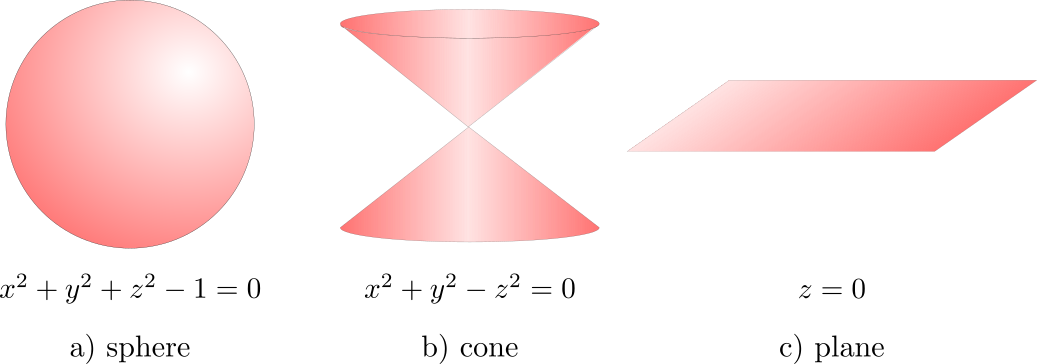
\includegraphics[scale=0.5]{images/img1}}
    \caption[Implicit surfaces with corresponding equations]
    {Implicit surfaces with corresponding equations.}
    %id obrazku, pomocou ktoreho sa budeme na obrazok odvolavat
    \label{img:1}
\end{figure}

Unit normal vector of the implicit surface in point $(x_0, y_0, z_0)$ is
normalized gradient of the implicit function in that point, provided it is
non-zero.

\begin{definition}
    Gradient vector of a function $F:\R^3 \to \R$ is defined as 
    $$\nabla F(x, y, z) = \bigg(\frac{\partial F(x, y, z)}{\partial x}, \frac{\partial F(x, y, z)}{\partial y}, 
    \frac{\partial F(x, y, z)}{\partial z}\bigg).$$
    If $\nabla F(x,y,z) \neq 0$, we can define the unit normal vector of $F$ as 
    a normalized gradient vector
    $$N(F(x, y, z))  = \frac{\nabla F(x, y, z)}{\| \nabla F(x, y, z) \|}.$$
    \\*
\end{definition}

Points lying on the implicit surface can be classified as regular or
singular based on the value of the gradient vector in that point.

\begin{definition}
    Point $P=(x,y,z)$ lying on the implicit surface is said to be regular,
    if $\nabla F(x, y, z) \neq 0$. On the contrary, point $P$ is said to be 
    singular, if $\nabla F(x, y, z) = 0$.
\end{definition}

Singular points can be further classified as isolated or non-isolated.

\begin{definition}
    Singular point $P$ of a surface $S$ is said to be isolated,
    if there exists an open ball $B_\varepsilon(P)$, which does not 
    contain any other singular point of $S$.
    Singular point $P$ is said to be non-isolated if it is not isolated.
\end{definition}

On the Figure \ref{img:2}, one can see an example of isolated and non-isolated
singularities.

\begin{figure}
    \centerline{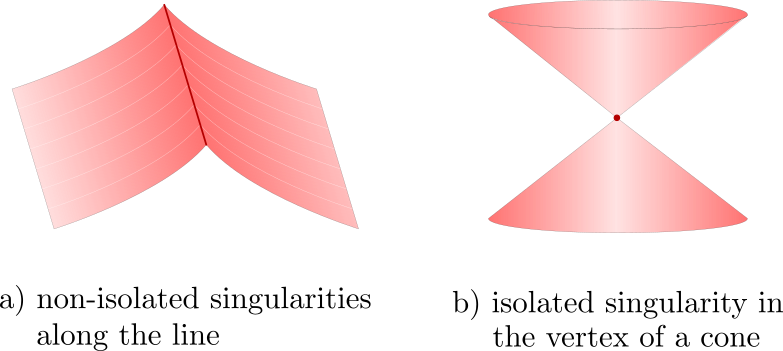
\includegraphics[scale=0.5]{images/img2}}
    \caption[Isolated and non-isolated singularity]
    {Isolated and non-isolated singularity.}
    %id obrazku, pomocou ktoreho sa budeme na obrazok odvolavat
    \label{img:2}
\end{figure}

\subsection{Curvature of a surface}

Curvature is a fundamental concept in differential geometry of curves and surfaces.
In case of curves, curvature is a measure of how much does the curve differ from a 
straight line. It is defined as the inverse of the radius of the osculating circle,
which is the second order approximation of the curve.

For surfaces, curvature is a measure of how much does the surface differ from a 
plane. The definition of the curvature of a surface is not as straightforward
as in the case of curves. The curvature of a curve on a surface depends on the 
choice of the tangent direction of a measured point.

The idea of measuring the curvature of a surface has a long history in mathematics.
One of the first contributors was a mathematician Carl Friedrich Gauss, who developed
the idea of the Gaussian curvature of surfaces. In this subsection, we are drawing from
the summary presented by Tiago Novello et al.\cite{novello2021differential}.

\subsubsection*{Normal curvature of the surface}

Let $S$ be a parametric surface $$S: D \subseteq \R^2 \to \R^3$$ 
$$S(u, v) = (S_x(u,v), S_y(u,v), S_z(u,v)), \hspace{3mm} (u,v)\in \R^2$$
Let the unit normal vector of the surface $S$ at the point $S(u, v)$ be $\vec{n}(u, v)$.

We define the normal curvature of the surface as a function of the location of the point
on the surface given by parameters $u$ and $v$ and the unit tangent vector in that point $\vec{u}$. 

\begin{definition}
Normal cut of a surface $S$ in the regular point $P$ in the direction of the unit tangent vector 
$\vec{u}$ is defined as an intersection of the surface $S$ and a plane
given by the vectors $\vec{u}$ and $\vec{n}(u, v)$ shifted to 
the point $S(u, v)$. 
\end{definition}

The visualisation of the normal cut is shown on the Figure \ref{img:14}.
It is clear, that the
normal cut is a plane curve lying on the surface, we denote this normal cut as $\nu_S(u, v, \vec{u})$.

\begin{figure}
    \centerline{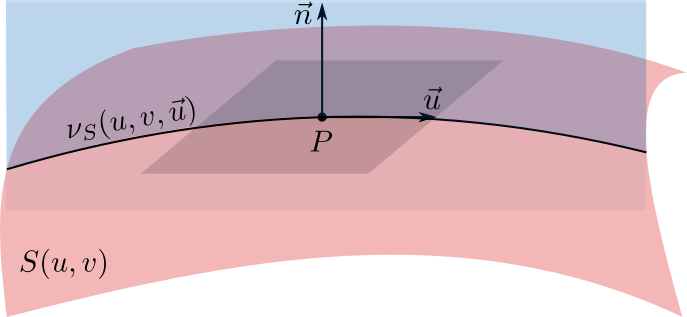
\includegraphics[scale=0.5]{images/img14}}
    \caption[Normal cut]
    {Normal cut of the parametric surface $S(u,v)$.}
    %id obrazku, pomocou ktoreho sa budeme na obrazok odvolavat
    \label{img:14}
\end{figure}

\begin{definition}
    Oriented normal curvature of the surface at the regular point $P$ in the direction of the unit tangent vector
    $\vec{u}$ is defined as the oriented curvature of the normal cut $\nu_S(u, v, \vec{u})$.
    Non-oriented normal curvature is defined as an absolute value of the oriented normal curvature.
\end{definition}

\begin{definition}
    Minimal and maximal curvature at the point $P = S(u,v)$ are defined as
    $$\kappa_{min}(u,v) = \min_{\vec{u} \in T_PS} \nu_S(u, v, \vec{u}),$$
    $$\kappa_{max}(u,v) = \max_{\vec{u} \in T_PS} \nu_S(u, v, \vec{u}),$$
    where $T_PS$ is a tangent plane of the surface $S$ in the point $P$.

    Minimal and maximal curvatures are called principal.
\end{definition}

\begin{definition}
    Gaussian curvature at a point $S(u, v)$ is defined as a product of principal curvatures
    at that point, i.e.
    $$\kappa_G(u, v) = \kappa_{min}(u,v) \kappa_{max}(u,v).$$
\end{definition}

Gaussian curvature describes the shape of the suface in the local neighborhood of the point.
Points of the surface S, where the Gaussian curvature is positive, are called elliptic.
Points of the surface S, where the Gaussian curvature is negative are called hyperbolic.
Points of the surface S, where only one of $\kappa_{min}, \kappa_{max}$ is zero, are called
parabolic and points, where both $\kappa_{min}$ and $\kappa_{max}$ are zero, are called planar.
The shape of the surface in the local neigborhoods of the points, visualized on the
Figure \ref{img:33}, is as follows:
\begin{itemize}
    \item {elliptic points $\longrightarrow$ sufrace is curved like an ellipsoid,}
    \item {hyperbolic points $\longrightarrow$ surface is curved like a saddle,}
    \item {parabolic points $\longrightarrow$ surface is curved like a parabolic cylinder,}
    \item {planar points $\longrightarrow$ surface is flat.}
\end{itemize}

\begin{figure}
    \centerline{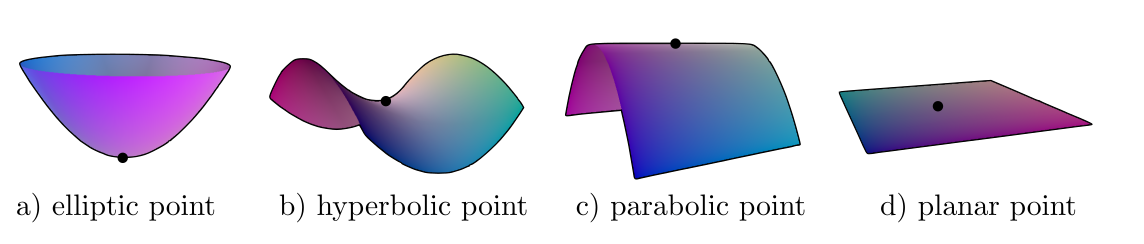
\includegraphics[scale=0.5]{images/img33}}
    \caption[Categorization of the surface points based on Gaussian curvature]
    {Categorization of the surface points based on Gaussian curvature \cite{morris2003client}.}
    %id obrazku, pomocou ktoreho sa budeme na obrazok odvolavat
    \label{img:33}
\end{figure}

Gaussian curvature is an
instrinsic propery, which means that it is also independent of the isometric image of the surface.

\begin{definition}
    Mean curvature of a surface $S$ at a point $P=S(u,v)$ is defined as an
    arithmetic mean of corresponding principal curvatures:
    $$\kappa_M(u, v) = \frac{\kappa_{min}(u,v) + \kappa_{max}(u,v)}{2}.$$
\end{definition}

Minimal, maximal, Gaussian and mean curvature are visualized in the Figure \ref{img:16},
where blue color indicates positive value of the corresponding visualized curvature,
red color indicates negative value of the corresponding visualized curvature
and white color indicates zero value of the corresponding visualized curvature.

\begin{figure}
    \centerline{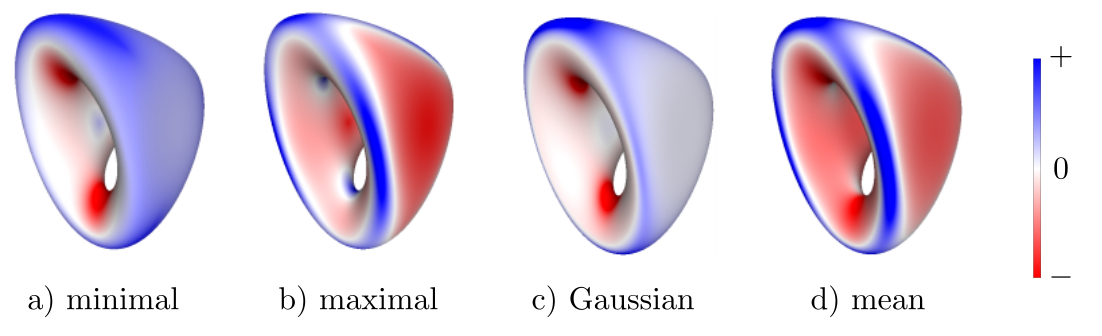
\includegraphics[scale=0.5]{images/img16}}
    \caption[Visualisation of the curvatures of the double-torus]
    {Visualisation of minimal, maximal, Gaussian and mean curvatures of the double-torus \cite{novello2021differential}.
    Blue/white/red color correspond to positive/zero/negative value of the corresponding curvature.}
    %id obrazku, pomocou ktoreho sa budeme na obrazok odvolavat
    \label{img:16}
\end{figure}

\subsection{Curvature formulas for implicit surface}

A version of curvature formulas for implicit surfaces appeared in \cite{spivak1975comprehensive}
and were reformulated, summarized and proved by Ron Goldman \cite{goldman2005curvature}.
In this subsection, we point out these formulas.

Let $F:\R^3 \to R$ be an implicit function which defines surface by the equation $F(x, y, z) = 0$. 
Let us denote $F_t = \frac{\partial F}{\partial t}$ and $F_{ts} = \frac{\partial^2 F}{\partial t \partial s}$.
Hessian matrix -- the matrix of the second order derivatives is defined as 
$$
H(F) = 
\begin{pmatrix}
    F_{xx} & F_{xy} & F_{xz} \\
    F_{yx} & F_{yy} & F_{yz} \\
    F_{zx} & F_{zy} & F_{zz}
\end{pmatrix},
$$
and the adjoint of the Hessian is defined as a transpose of its cofactor matrix.
$$
H^*(F) = 
\begin{pmatrix}
    \begin{vmatrix} F_{yy} & F_{yz} \\ F_{zy} & F_{zz} \end{vmatrix} & 
    -\begin{vmatrix} F_{xy} & F_{xz} \\ F_{zy} & F_{zz} \end{vmatrix} &
    \begin{vmatrix} F_{xy} & F_{xz} \\ F_{yy} & F_{yz} \end{vmatrix} \\

    -\begin{vmatrix} F_{yx} & F_{yz} \\ F_{zx} & F_{zz} \end{vmatrix} &
    \begin{vmatrix} F_{xx} & F_{xz} \\ F_{zx} & F_{zz} \end{vmatrix} & 
    -\begin{vmatrix} F_{xx} & F_{xz} \\ F_{yx} & F_{yz} \end{vmatrix} \\

    \begin{vmatrix} F_{yx} & F_{yy} \\ F_{zx} & F_{zy} \end{vmatrix} & 
    -\begin{vmatrix} F_{xx} & F_{xy} \\ F_{zx} & F_{zy} \end{vmatrix} & 
    \begin{vmatrix} F_{xx} & F_{xy} \\ F_{yx} & F_{yy} \end{vmatrix}
\end{pmatrix}.
$$

Now, one can find the formulas of Gaussian, mean, minimal and maximal curvature
for an implicit surface $F=0$ at a regular point.

Gaussian curvature is given by 
$$\kappa_G = \frac{\nabla F \cdot H^*(F) \cdot \nabla F^T}{|\nabla F|^4}.$$

Mean curvature of the implicit surface defined by function $F$ is given by 
$$\kappa_M = \frac{\nabla F \cdot H^*(F) \cdot \nabla F^T - | \nabla F |^2 Tr(H)}{2|\nabla F|^3}.$$

The principal curvatures $\kappa_{min}$ and $\kappa_{max}$ can be calculated from Gaussian curvature and
mean curvature as 
$$\kappa_{min}, \kappa_{max} = \kappa_M \pm \sqrt{\kappa_M^2-\kappa_G}.$$

\section{ADE singularities}
\label{sub2.2}

ADE singularities, also reffered to as du Val singularities are a specific
class of simple, isolated surface singularities.
They were classified by Arnold's
\cite{arnol1972normal} according to ADE classification
\cite{hazewinkel1977ubiquity} based on
correspondence of these singualrities to simply laced Dynkin diagrams
\cite{dynkin1947structure}.
We know infinitely many $A$ singularities -- $A_1, A_2, ...$,
infinitely many $D$ singularities -- $D_4, D_5, ...$ and three $E$
singularities -- $E_6, E_7$ and $E_8$.
ADE singularities are specified by their normal forms.
When working in complex space, each singularity has a single normal form:
\begin{itemize}
    \item $A_n$ \hspace{5mm} $F(x,y,z)=x^{n+1}+y^2+z^2$,
    \item $D_n$ \hspace{5mm} $F(x,y,z)=yx^2+y^{n-1}+z^2$,
    \item $E_6$ \hspace{5mm} $F(x,y,z)=x^3+y^4+z^2$,
    \item $E_7$ \hspace{5mm} $F(x,y,z)=x^3+xy^3+z^2$,
    \item $E_8$ \hspace{5mm} $F(x,y,z)=x^3+y^5+z^2$.
\end{itemize}

Each ADE singularity on a surface can be locally expressed by their
normal form.

In the real case, changing the signs in these equations produces different
surfaces and therefore, ADE singualrities can be further classified by their
signature.

\begin{definition}
    Let real surface singularities based on their signature be denoted as follows:
    \begin{itemize}
        \item $A_{n\pm\pm}$ \hspace{5mm} $F(x,y,z)=x^{n+1}\pm y^2\pm z^2$,
              
        \item $D_{n\pm\pm}$ \hspace{5mm} $F(x,y,z)=yx^2\pm y^{n-1}\pm z^2$,
        
        \item $E_{6\pm\pm}$ \hspace{5mm} $F(x,y,z)=x^3\pm y^4\pm z^2$,
        
        \item $E_{7\pm\pm}$ \hspace{5mm} $F(x,y,z)=x^3\pm xy^3\pm z^2$,
        
        \item $E_{8\pm\pm}$ \hspace{5mm} $F(x,y,z)=x^3\pm y^5\pm z^2$.
        \end{itemize}
\end{definition}

The most common example of a surface with ADE singularity is an ordinary cone.
Given as the zero set of the function $F(x, y, z)=x^2-y^2-z^2$, cone has
a singular point $P=(0, 0, 0)$. This singular point is an example of $A_{1--}$
singularity.

\subsection{Correspondence between $SO(3,\R)$ group and ADE singularities}
\label{subs2.2.2}
$SO(3, \R)$ is special orthogonal group over the field of real numbers 
in three dimensions. It is also called $3D$ rotation group, as it is a group
of all rotations around axes passing through the origin in $R^3$.
\begin{definition}
    $SO(3, \R)$ is a group of $3\times3$ orthogonal matrices
    of real numbers with determinant $1$.
    $$SO(3, \R) = \bigg\{A\in\R^{3\times3} \hspace{1mm} | AA^T=I ,\hspace{1mm} det(A)=1\bigg\}.$$
\end{definition}

Simply laced Dynkin diagrams correspond to all finite subgroups of
$SO(3,\R)$. Finite subgroups of
$SO(3,\R)$ are the rotational symmetry groups of
\begin{itemize}
    \item pyramid with $n$ vertices (cyclic subgroup $\overline{C}_n$) -- Figure \ref{img:34} a),
    \item double pyramid with $n$ vertices (dihedral subgroup $\overline{D}_n$) -- Figure \ref{img:34} b),
    \item platonic solids:
    \begin{itemize}
        \item tetrahedron (tetrahedral subgroup $\overline{T}$) -- Figure \ref{img:34} c),
        \item octahedron (octahedral subgroup $\overline{O}$) -- Figure \ref{img:34} d),
        \item icosahedron (icosahedral subgroup $\overline{I}$) -- Figure \ref{img:34} e).
    \end{itemize}
\end{itemize}

\begin{figure}
    \centerline{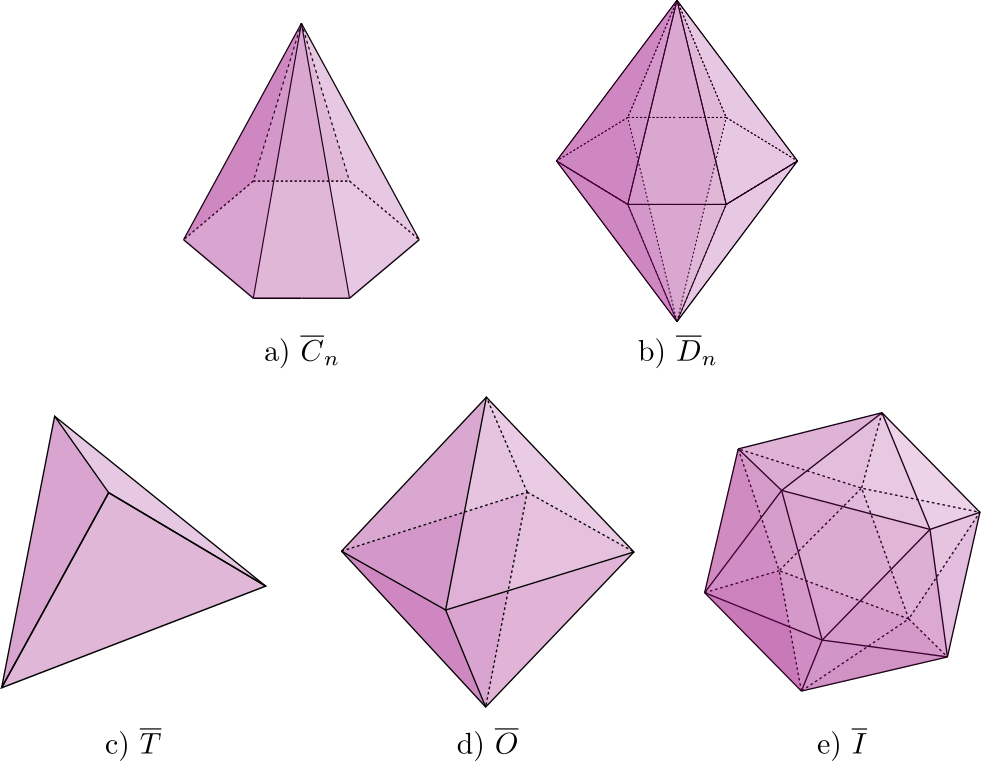
\includegraphics[scale=0.5]{images/img34}}
    \caption[Shapes representing the $SO(3,\R)$ group]
    {Shapes representing the $SO(3,\R)$ group.}
    %id obrazku, pomocou ktoreho sa budeme na obrazok odvolavat
    \label{img:34}
\end{figure}

The correspondence is as follows:
\begin{itemize}
    \item $A_n \iff \overline{C}_{n+1}$,
    \item $D_n \iff \overline{D}_{n+2}$,
    \item $E_6 \iff \overline{T}$,
    \item $E_7 \iff \overline{O}$,
    \item $E_8 \iff \overline{I}$.
\end{itemize}

The conclusion is that ADE singularities correspond to finite subgroups of
$SO(3, \R)$, which represent certain types of symmetries in $\R^3$.

\section{CSG modelling for implcit surfaces}
\label{sub2.6}
In this section we will discuss how constructive solid geometry can be used for
modelling complex implicit surfaces. First major publication regarding constructive
solid geometry was published in 1977 by Requicha and Voelcker \cite{requicha1977constructive}.
More detailed mathematical foundations were published a year later, in 1978 by
Requicha and Tilove \cite{requicha1978mathematical}.
\subsection{Constructive solid geometry (CSG)}
Constructive solid geometry is a technique used for modelling complex geometric
objects using boolean operations on sets of points -- union, intersection and
difference. It gained populatity in 1980s as a powerful tool to create complex
shapes from sets of geometrical primitives, such as cylinders, spheres and cones.
The resulting model can be represented as a CSG tree, which contains geometrical
primitives in its leaves and boolean operations in its internal nodes 
\cite{foley1996computer}. An example of such CSG tree can be seen on the Figure 
\ref{img:18}.

\begin{figure}
    \centerline{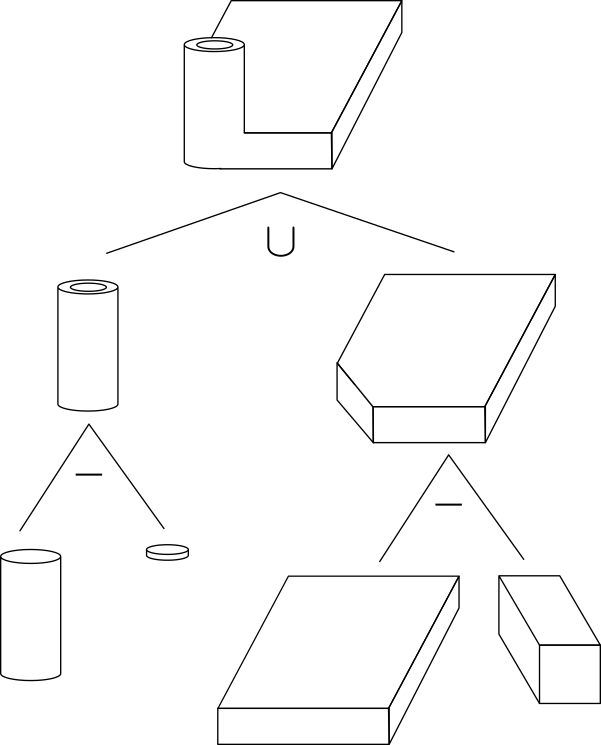
\includegraphics[scale=0.5]{images/img18}}
    \caption[Example of CSG tree]
    {Example of CSG tree \cite{foley1996computer}.}
    %id obrazku, pomocou ktoreho sa budeme na obrazok odvolavat
    \label{img:18}
\end{figure}

\subsubsection*{CSG for implcit surfaces}
As the implicit surface divides space into inside $(F(x, y, z) < 0)$ and
outside $(F(x, y, z) > 0)$, one can easily combine the idea of
implicit surfaces and CSG modelling. Given two implicit surfaces represented
by implicit functions $F$ and $G$, the surface of the
intersection of the interiors can be defined by implicit fuction $H=min(F, G)$.
Similarly, the surface of the union of the interiors can be defined
by implicit function $H=max(F, G)$ and lastly, the surface of the difference of
the interiors can be defined by implicit function $H=max(F, -G)$. Two dimensional
example of this idea can be seen on the Figure \ref{img:19}.

\begin{figure}
    \centerline{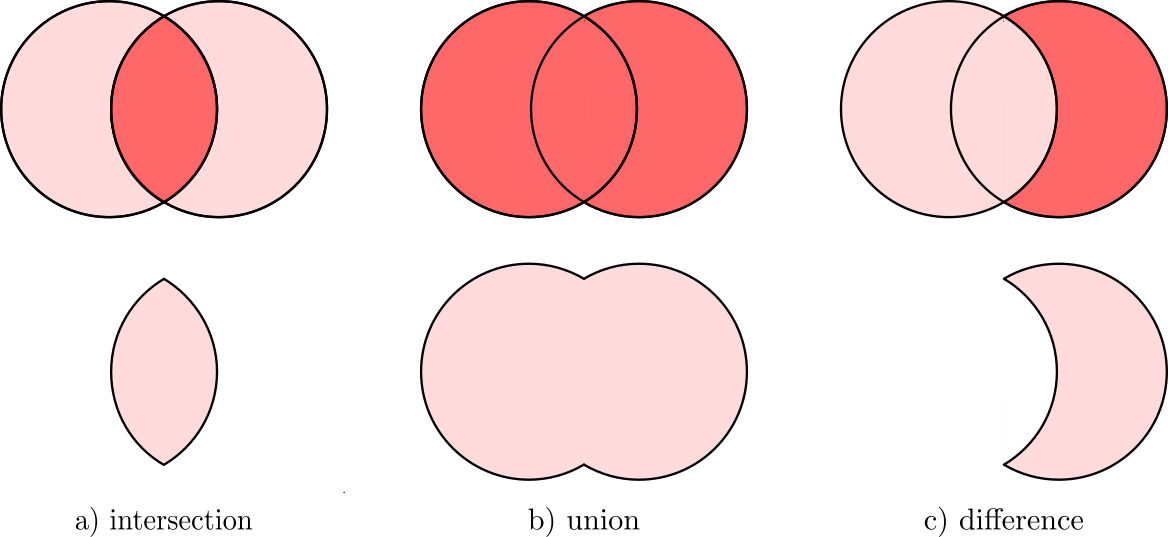
\includegraphics[scale=0.5]{images/img19}}
    \caption[Boolean operations on implicit curves]
    {Boolean operations on implicit curves.}
    %id obrazku, pomocou ktoreho sa budeme na obrazok odvolavat
    \label{img:19}
\end{figure}

\begin{theorem}
    The minimum function $min(F, G)$ of two functions $F:\R^3 \to \R$ and
    $G:\R^3 \to \R$ is defined as $$min(F, G) = F + G - \sqrt{F^2+G^2}$$.
    The maximum function $max(F, G)$ of two functions $F:\R^3 \to \R$ and
    $G:\R^3 \to \R$ is defined as $$max(F, G) = F + G + \sqrt{F^2+G^2}$$.
\end{theorem}

These formulas allow us to model implicit surfaces which are the result of
performing finite number of operations union, intersection and difference
on arbitrary implicit functions.

An easy example is creating an implicit equation representing a half of
a sphere. Let us have an implicit function 
$F(x, y, z) = x^2+y^2+z^2-1$, which represents a unit sphere and another
implicit function $G(x, y, z) = z$ which represents the $xy$ plane.
The minimum function of these two functions
$$min(F, G) = x^2+y^2+y^2-1+z-\sqrt{(x^2+y^2+y^2-1)^2+z^2}$$ represents the
surface of a half sphere. The visualisation of these surfaces can be seen on
the Figure \ref{img:20}.
\begin{figure}
    \centerline{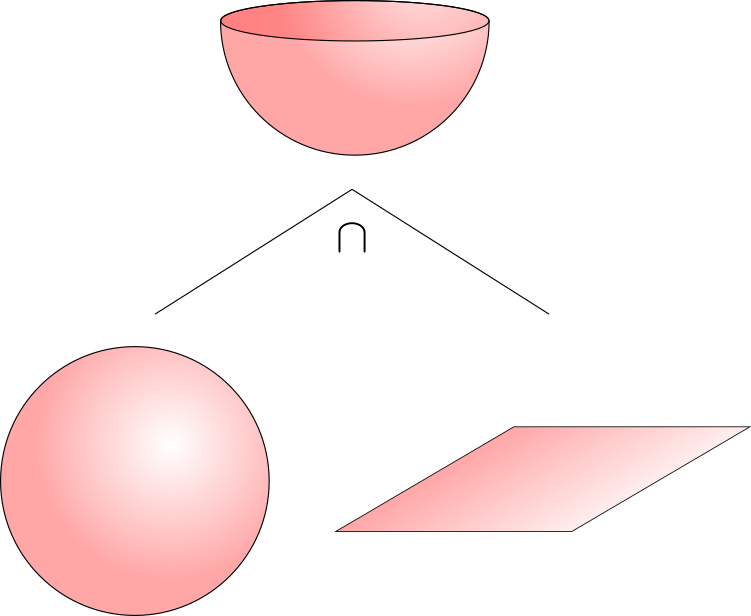
\includegraphics[scale=0.5]{images/img20}}
    \caption[Intersection of a sphere and a plane]
    {Intersection of a sphere and a plane.}
    %id obrazku, pomocou ktoreho sa budeme na obrazok odvolavat
    \label{img:20}
\end{figure}


\section{Non-isolated surface singularities}
\label{sub2.3}

As we already mentioned, non-isolated singular point of the surface $S$ is 
the singular point, for which
every open ball $B_\varepsilon(P)$ contains other singular points of the surface $S$.
Non-isolated singular points are also called singular curves.

In the CSG modelling, singular curves most commonly arise as a result of intersection,
union and difference operations on the interiors of these surfaces. When performing
the intersection, union or difference operation on the interiors of two regular surfaces, 
the singular curve is the curve given by the intersection of these surfaces. An example
of an intersection of two spherical interiors is shown on the Figure \ref{img:35}, 
the resulting singular curve given by an intersection of the two speres is displayed
by the red color.

\begin{figure}
    \centerline{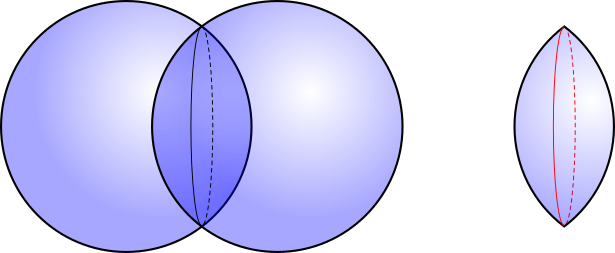
\includegraphics[scale=0.5]{images/img35}}
    \caption[Intersection of a two spheres]
    {Intersection of a two spheres.}
    %id obrazku, pomocou ktoreho sa budeme na obrazok odvolavat
    \label{img:35}
\end{figure}

\subsubsection{Projecting point to the implicit curve}

Implicit curve $C$ is given by two implicit equations - the equations of two surfaces
which intersect in the curve $C$.
To project a point close to the surface to the given surface, we use the method where
we project the point in the direction of the normal vector using the iterative 
Newton-Rhapson method. An extension of this method can be used to project a point
to the implicit curve, by alternately projecting to the two surfaces until the
point lies on both with required precision. A visualization of this approach can be
seen on the image \ref{img:36}. We denote the projection function $proj_C$.

\begin{figure}
    \centerline{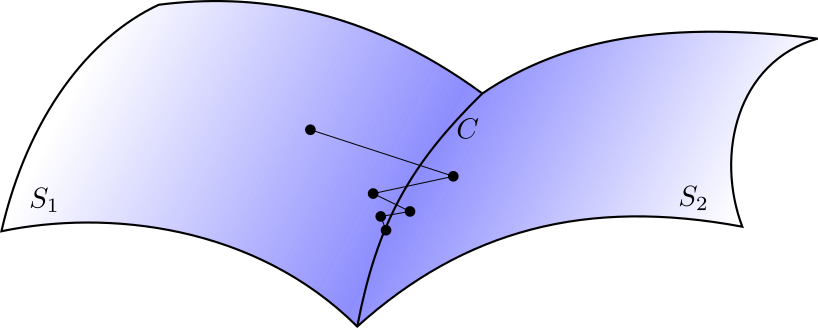
\includegraphics[scale=0.5]{images/img36}}
    \caption[Projecting a point to the implicit curve]
    {Projecting a point to the implicit curve.}
    %id obrazku, pomocou ktoreho sa budeme na obrazok odvolavat
    \label{img:36}
\end{figure}

\subsubsection {Differential geometry of implicit curves}

An implicit curve $C$ is
given by two implicit equations $F_1, F_2: \R^3 \to \R$ representing two implicit
surfaces $S_1$ and $S_2$, respectively which are intersecting in the implicit 
curve $C$. The unit tangent vector $\vec{t}_C$  
of the curve $C$ in the point $P \in C$ is given by the cross product of 
unit normal vectors of the surfaces $S_1$ and $S_2$
$$\vec{t}_C(P) = \vec{n}_{S_1}(P) \times \vec{n}_{S_1}(P).$$
